
\addcontentsline{toc}{chapter}{Moulakhass}

\begin{figure}[H]
    \thispagestyle{plain}
    \centering
    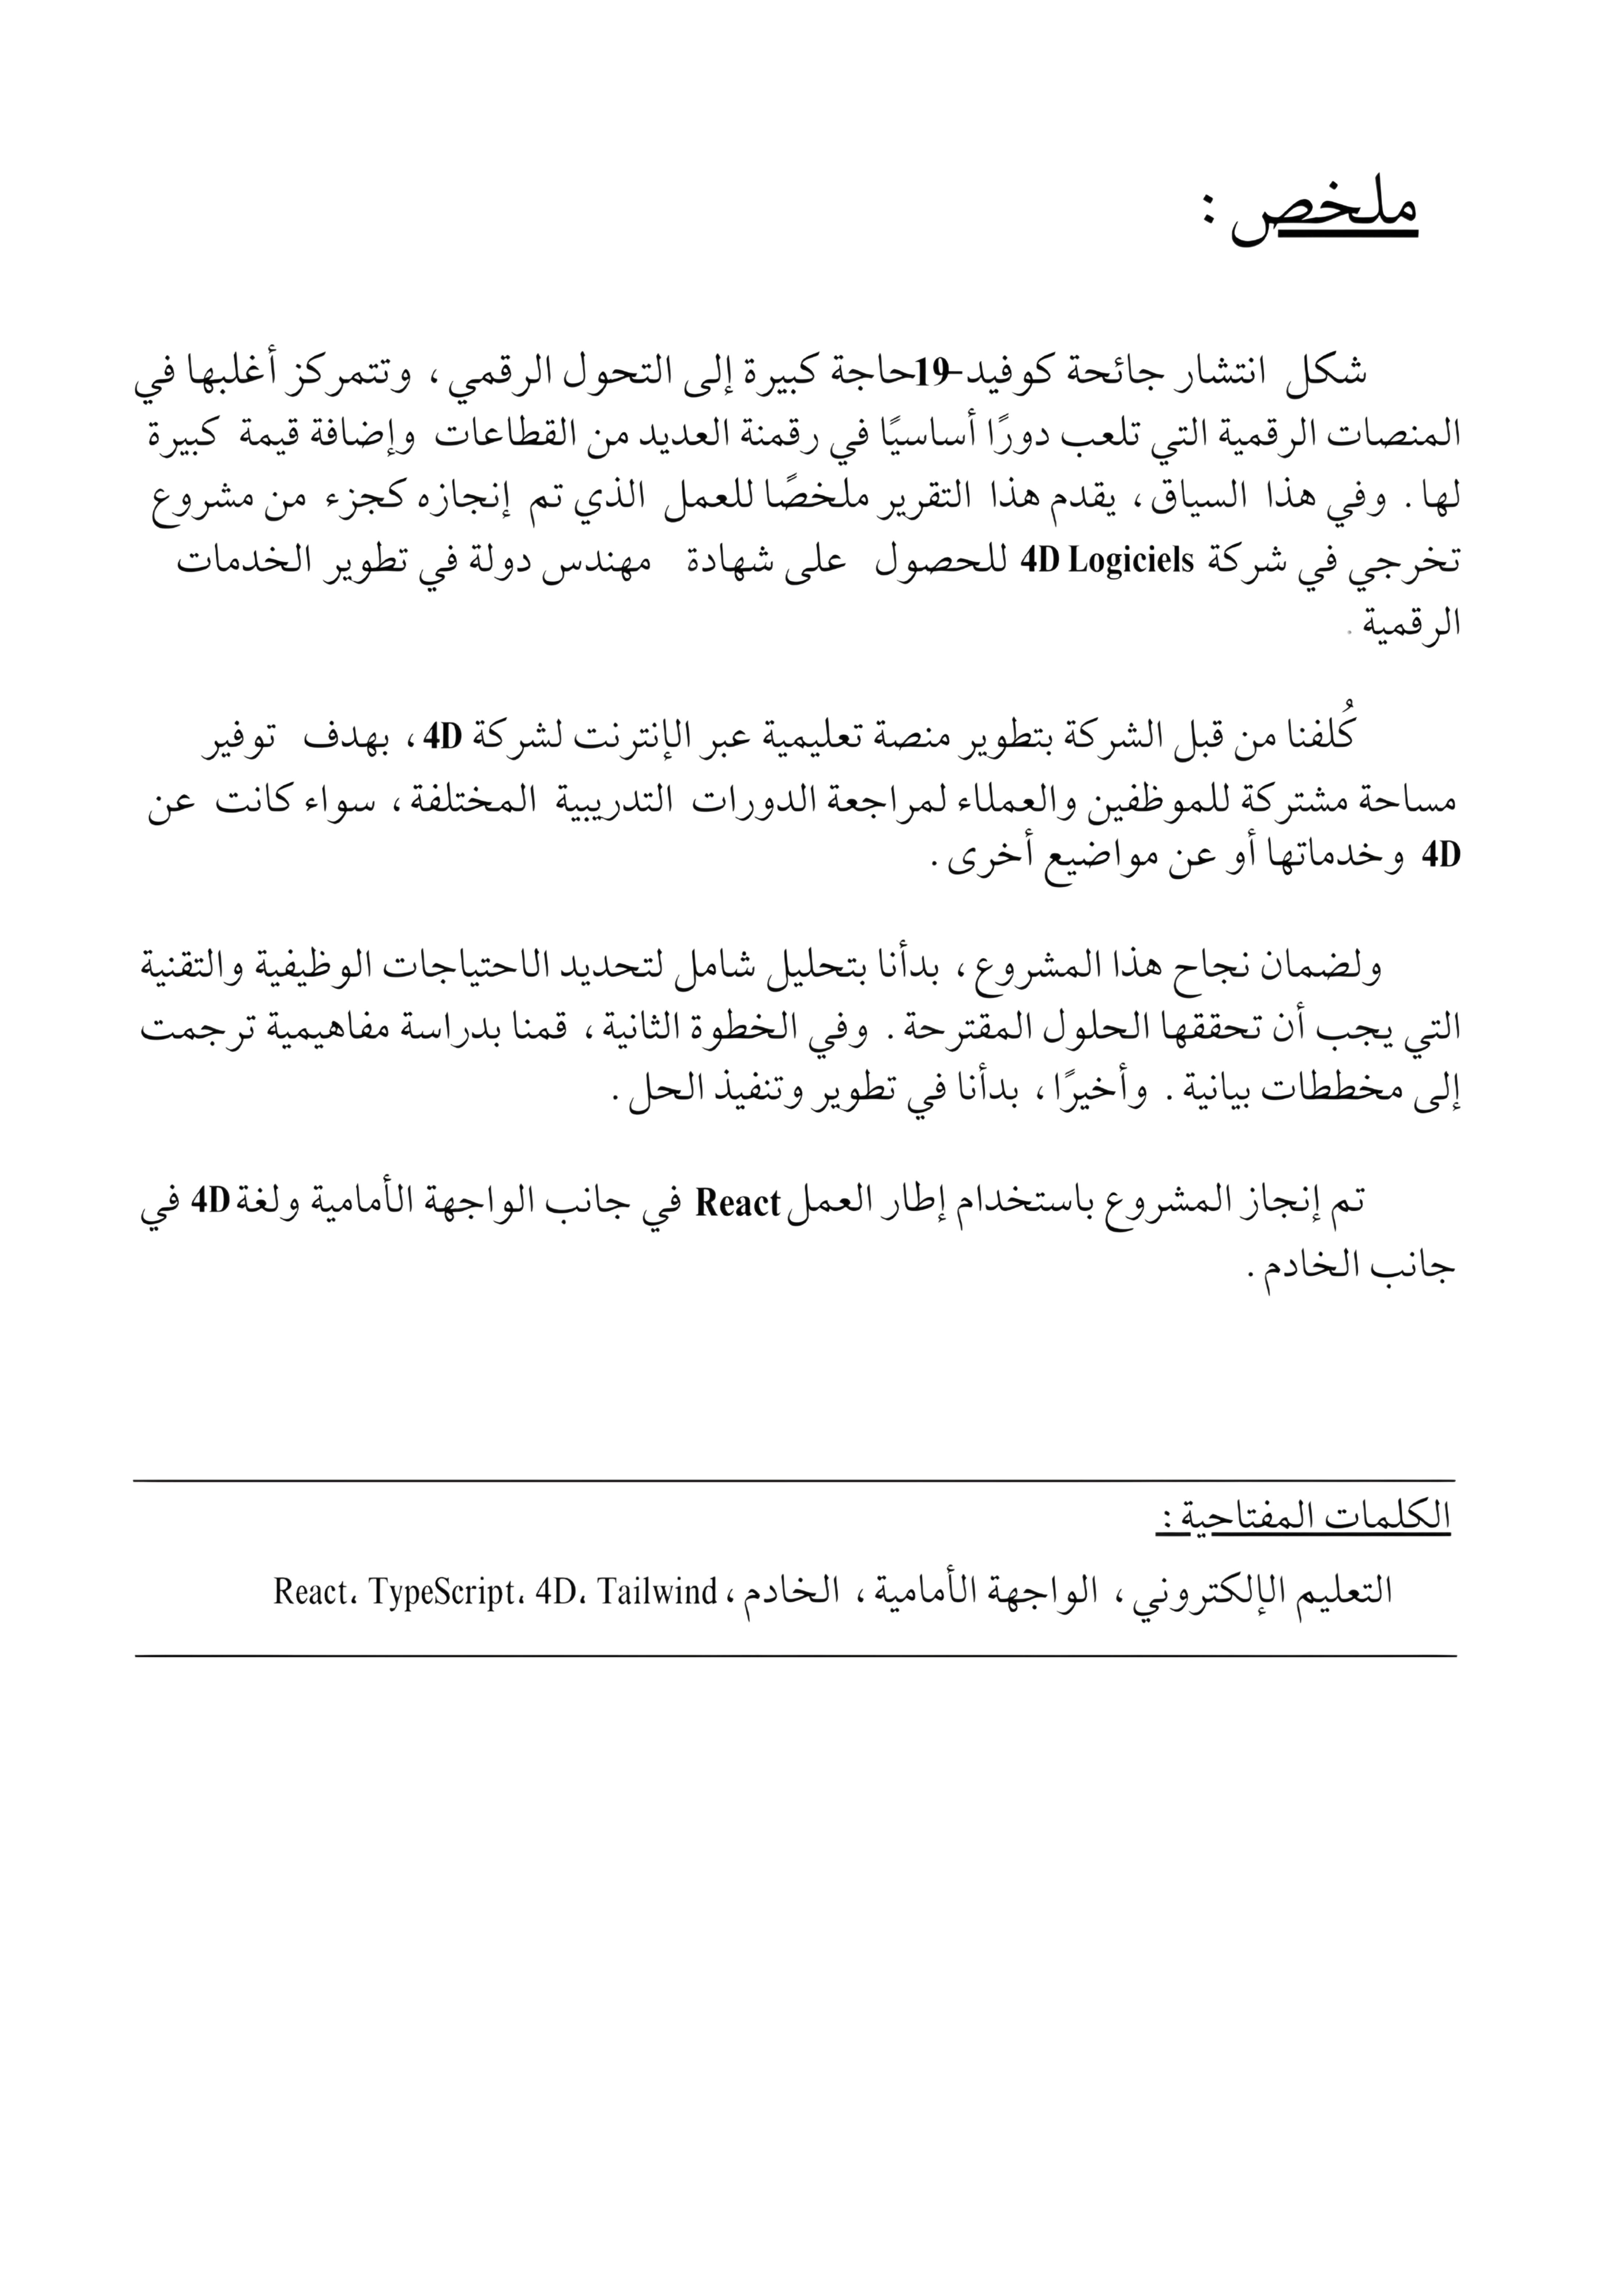
\includegraphics[width=19cm]{Figures/abstract.png}
\end{figure}


\newpage

\chapter*{Résumé}
\addcontentsline{toc}{chapter}{Résumé}


De nos jours, la demande pour la transformation digitale ne cesse de croître, surtout après la pandémie de COVID-19. Dans ce contexte, les plateformes numériques jouent un rôle primordial en numérisant de nombreux secteurs d'activité et en créant de la valeur.
\vspace{10pt}

Ce document présente la synthèse du travail réalisé dans le cadre de mon projet de fin d’études au sein de la société 4D Logiciels pour l’obtention du diplôme d’ingénieur d’état en développement des services numériques.

\vspace{10pt}

Nous avons été chargés par l’entreprise de développer une plateforme de formation en ligne pour 4D. Ce projet interne de l’entreprise vise à fournir aux employés de la société ainsi qu'aux clients un espace partagé où ils peuvent consulter les différentes formations, qu’elles portent sur 4D ou sur d’autres sujets.

\vspace{10pt}

Pour réussir ce projet, nous avons commencé par une analyse approfondie du projet dans le but d’identifier les besoins fonctionnels et techniques, auxquels la solution doit répondre. Dans une seconde étape, nous avons mené une étude conceptuelle traduite en diagrammes. Finalement, nous avons initié le développement et la mise en œuvre de la solution.

\vspace{10pt}

Le projet a été mis en œuvre en utilisant le Framework React coté Frontend et le langage 4D pour le Backend.

\vspace{10pt}


\noindent\rule[2pt]{\textwidth}{0.5pt}

{\textbf{Mots clés :}}
E-learning, Frontend, Backend, React, typescript, 4D, Tailwind.
\\
\noindent\rule[2pt]{\textwidth}{0.5pt}